% Options for packages loaded elsewhere
\PassOptionsToPackage{unicode}{hyperref}
\PassOptionsToPackage{hyphens}{url}
\PassOptionsToPackage{dvipsnames,svgnames,x11names}{xcolor}
\PassOptionsToPackage{space}{xeCJK}
\documentclass[
  11pt,
  a4paper,
]{article}
\usepackage{xcolor}
\usepackage[margin=2.2cm]{geometry}
\usepackage{amsmath,amssymb}
\setcounter{secnumdepth}{-\maxdimen} % remove section numbering
\usepackage{iftex}
\ifPDFTeX
  \usepackage[T1]{fontenc}
  \usepackage[utf8]{inputenc}
  \usepackage{textcomp} % provide euro and other symbols
\else % if luatex or xetex
  \usepackage{unicode-math} % this also loads fontspec
  \defaultfontfeatures{Scale=MatchLowercase}
  \defaultfontfeatures[\rmfamily]{Ligatures=TeX,Scale=1}
\fi
\usepackage{lmodern}
\ifPDFTeX\else
  % xetex/luatex font selection
  \setmainfont[]{Microsoft YaHei}
  \ifXeTeX
    \usepackage{xeCJK}
    \setCJKmainfont[]{Microsoft YaHei}
  \fi
  \ifLuaTeX
    \usepackage[]{luatexja-fontspec}
    \setmainjfont[]{Microsoft YaHei}
  \fi
\fi
% Use upquote if available, for straight quotes in verbatim environments
\IfFileExists{upquote.sty}{\usepackage{upquote}}{}
\IfFileExists{microtype.sty}{% use microtype if available
  \usepackage[]{microtype}
  \UseMicrotypeSet[protrusion]{basicmath} % disable protrusion for tt fonts
}{}
\makeatletter
\@ifundefined{KOMAClassName}{% if non-KOMA class
  \IfFileExists{parskip.sty}{%
    \usepackage{parskip}
  }{% else
    \setlength{\parindent}{0pt}
    \setlength{\parskip}{6pt plus 2pt minus 1pt}}
}{% if KOMA class
  \KOMAoptions{parskip=half}}
\makeatother
\usepackage{longtable,booktabs,array}
\newcounter{none} % for unnumbered tables
\usepackage{calc} % for calculating minipage widths
% Correct order of tables after \paragraph or \subparagraph
\usepackage{etoolbox}
\makeatletter
\patchcmd\longtable{\par}{\if@noskipsec\mbox{}\fi\par}{}{}
\makeatother
% Allow footnotes in longtable head/foot
\IfFileExists{footnotehyper.sty}{\usepackage{footnotehyper}}{\usepackage{footnote}}
\makesavenoteenv{longtable}
\usepackage{graphicx}
\makeatletter
\newsavebox\pandoc@box
\newcommand*\pandocbounded[1]{% scales image to fit in text height/width
  \sbox\pandoc@box{#1}%
  \Gscale@div\@tempa{\textheight}{\dimexpr\ht\pandoc@box+\dp\pandoc@box\relax}%
  \Gscale@div\@tempb{\linewidth}{\wd\pandoc@box}%
  \ifdim\@tempb\p@<\@tempa\p@\let\@tempa\@tempb\fi% select the smaller of both
  \ifdim\@tempa\p@<\p@\scalebox{\@tempa}{\usebox\pandoc@box}%
  \else\usebox{\pandoc@box}%
  \fi%
}
% Set default figure placement to htbp
\def\fps@figure{htbp}
\makeatother
\setlength{\emergencystretch}{3em} % prevent overfull lines
\providecommand{\tightlist}{%
  \setlength{\itemsep}{0pt}\setlength{\parskip}{0pt}}
\setCJKmonofont{Microsoft YaHei}
\setlength{\emergencystretch}{3em}
\usepackage{needspace}
\usepackage{bookmark}
\IfFileExists{xurl.sty}{\usepackage{xurl}}{} % add URL line breaks if available
\urlstyle{same}
\hypersetup{
  pdftitle={协程技术调研报告},
  pdfauthor={并行程序设计课程调研},
  colorlinks=true,
  linkcolor={blue},
  filecolor={Maroon},
  citecolor={Blue},
  urlcolor={blue},
  pdfcreator={LaTeX via pandoc}}

\title{协程技术调研报告}
\usepackage{etoolbox}
\makeatletter
\providecommand{\subtitle}[1]{% add subtitle to \maketitle
  \apptocmd{\@title}{\par {\large #1 \par}}{}{}
}
\makeatother
\subtitle{从并发模型演进、运行时机制到本地 TCP I/O 实验验证}
\author{并行程序设计课程调研}
\date{2026-05-26}

\begin{document}
\maketitle

\section{摘要}\label{ux6458ux8981}

协程（coroutine）是一种降低等待资源成本的并发抽象，主要用于减少大量 I/O
等待任务对 OS
线程的长期占用。现代云服务中，请求经常在等待网络、数据库、RPC
下游、缓存、消息队列或定时器；如果每个请求都绑定一个平台线程，那么线程栈、线程对象、上下文切换和调度成本会随着并发数增加而放大。

本报告围绕四个问题展开：

\begin{enumerate}
\def\labelenumi{\arabic{enumi}.}
\tightlist
\item
  并发执行机制为什么会从进程、线程、事件循环演进到协程；
\item
  协程在底层如何实现，包括状态机、协程帧、挂起与恢复；
\item
  C++20、Go、Python、C\#、Java 21 对协程或轻量并发的支持有何差异；
\item
  本地实验如何验证协程在 I/O 等待场景中的资源优势，以及它在 CPU
  密集场景中的边界。
\end{enumerate}

核心结论如下：

\begin{itemize}
\tightlist
\item
  协程的主要价值是降低 I/O
  等待任务的线程占用；其他任务类型仍需选择匹配其瓶颈的执行模型。
\item
  操作系统仍然调度真实线程；协程由语言、编译器和运行时在用户态组织。
\item
  不同语言的``协程''抽象层级不同，工程评估需要结合运行时、调度模型和异步生态。
\item
  本地 TCP I/O 实验显示，\texttt{asyncio} 能用 0 个业务新增线程承载 5000
  个 TCP 请求；线程池可以通过增加 worker
  获得更低耗时，但代价是显著增加业务线程和 RSS 增量。
\item
  CPU-bound 实验显示，协程调度不增加 CPU 算力。CPU
  密集任务应使用进程池、原生扩展、向量化、SIMD 或 GPU 等并行计算方案。
\end{itemize}

\section{1.
并发模型为什么演进到协程}\label{ux5e76ux53d1ux6a21ux578bux4e3aux4ec0ux4e48ux6f14ux8fdbux5230ux534fux7a0b}

\subsection{1.1
高并发服务的瓶颈常常是等待}\label{ux9ad8ux5e76ux53d1ux670dux52a1ux7684ux74f6ux9888ux5e38ux5e38ux662fux7b49ux5f85}

在很多服务端程序中，一个请求的大部分时间花在等待外部事件上，CPU
计算通常只占较短片段：

\begin{itemize}
\tightlist
\item
  等待客户端网络包到达；
\item
  等待数据库、Redis、消息队列或 RPC 下游响应；
\item
  等待磁盘、对象存储或文件系统；
\item
  等待连接池、限流器、定时器或锁。
\end{itemize}

如果使用``一个请求一个线程''的模型，阻塞等待期间线程本身并没有执行有意义的计算，但线程栈、调度上下文和内核对象仍然存在。当并发数达到几千甚至几万时，线程资源开销会成为限制系统扩展性的因素。

早期的 C10K
问题集中讨论了单机同时处理一万个客户端连接的挑战。它推动了事件驱动服务器、非阻塞
I/O、\texttt{epoll}/\texttt{kqueue}/IOCP、异步框架和协程运行时的发展。现代协程技术可以看作是这一演进链路上的重要抽象：它试图同时保留事件驱动的资源效率和同步代码的可读性。

\subsection{1.2
从进程到协程的演进逻辑}\label{ux4eceux8fdbux7a0bux5230ux534fux7a0bux7684ux6f14ux8fdbux903bux8f91}

{\def\LTcaptype{none} % do not increment counter
\begin{longtable}[]{@{}
  >{\raggedright\arraybackslash}p{(\linewidth - 6\tabcolsep) * \real{0.2500}}
  >{\raggedright\arraybackslash}p{(\linewidth - 6\tabcolsep) * \real{0.2500}}
  >{\raggedright\arraybackslash}p{(\linewidth - 6\tabcolsep) * \real{0.2500}}
  >{\raggedright\arraybackslash}p{(\linewidth - 6\tabcolsep) * \real{0.2500}}@{}}
\toprule\noalign{}
\begin{minipage}[b]{\linewidth}\raggedright
阶段
\end{minipage} & \begin{minipage}[b]{\linewidth}\raggedright
核心模型
\end{minipage} & \begin{minipage}[b]{\linewidth}\raggedright
主要收益
\end{minipage} & \begin{minipage}[b]{\linewidth}\raggedright
主要问题
\end{minipage} \\
\midrule\noalign{}
\endhead
\bottomrule\noalign{}
\endlastfoot
多进程 & 一个请求或一组请求由进程处理 & 隔离强，崩溃影响小 &
创建、切换、内存成本高 \\
多线程 & 一个请求绑定一个线程 & 代码直观，共享内存方便 &
大量线程带来栈内存和调度开销 \\
事件循环 & 少量线程处理大量事件 & 线程少，I/O 吞吐高 &
回调链复杂，状态分散 \\
async/await 协程 & 用顺序代码表达异步等待 & 兼顾性能和可读性 &
需要非阻塞生态，阻塞调用会破坏调度 \\
虚拟线程/轻量线程 & 用近似线程的 API 表达高并发任务 &
迁移成本低，工程心智简单 & 仍有运行时调度、pinning、下游容量等边界 \\
\end{longtable}
}

这一演进体现了不同抽象对不同瓶颈的适配关系。工程选型应先识别任务瓶颈，再选择执行模型。

\begin{itemize}
\tightlist
\item
  CPU 密集任务需要真正并行，重点是多核、进程池、原生扩展、SIMD、GPU。
\item
  I/O 密集任务重点是减少等待时占用的 OS 线程，协程和异步 I/O 更合适。
\item
  强隔离任务仍然适合进程。
\item
  传统同步服务端代码迁移可考虑 Java 虚拟线程这类轻量线程化抽象。
\end{itemize}

\section{2.
协程的底层机制}\label{ux534fux7a0bux7684ux5e95ux5c42ux673aux5236}

\subsection{2.1
协程是可暂停、可恢复的函数}\label{ux534fux7a0bux662fux53efux6682ux505cux53efux6062ux590dux7684ux51fdux6570}

普通函数调用后会沿调用栈连续执行到返回；协程函数可以在挂起点保存当前状态，然后把执行权交还给调度器，之后再从挂起点继续执行。

一个协程系统通常包含：

\begin{itemize}
\tightlist
\item
  协程函数：例如
  \texttt{async\ def}、\texttt{async}、\texttt{co\_await}、\texttt{go}；
\item
  协程对象或任务对象：代表一次尚未完成的异步执行；
\item
  挂起点：例如 \texttt{await}、\texttt{yield}、channel 阻塞、sleep、I/O
  等待；
\item
  调度器：决定哪个可运行协程继续执行；
\item
  事件源：网络 I/O、定时器、文件 I/O、锁、Future 完成等。
\end{itemize}

通俗地说，协程把一个连续执行的函数拆成多个片段。每当执行到
\texttt{await}
这类挂起点，如果等待对象尚未完成，当前函数的局部变量、下一条指令位置、返回值、异常信息等会被保存到协程帧或状态机对象中，运行时可以去执行其他任务。

\subsection{2.2 Stackless 与 Stackful}\label{stackless-ux4e0e-stackful}

协程实现大体可分为两类。

{\def\LTcaptype{none} % do not increment counter
\begin{longtable}[]{@{}
  >{\raggedright\arraybackslash}p{(\linewidth - 4\tabcolsep) * \real{0.3333}}
  >{\raggedright\arraybackslash}p{(\linewidth - 4\tabcolsep) * \real{0.3333}}
  >{\raggedright\arraybackslash}p{(\linewidth - 4\tabcolsep) * \real{0.3333}}@{}}
\toprule\noalign{}
\begin{minipage}[b]{\linewidth}\raggedright
类型
\end{minipage} & \begin{minipage}[b]{\linewidth}\raggedright
特点
\end{minipage} & \begin{minipage}[b]{\linewidth}\raggedright
代表
\end{minipage} \\
\midrule\noalign{}
\endhead
\bottomrule\noalign{}
\endlastfoot
Stackless coroutine &
不保存完整调用栈，编译器把函数拆成状态机，局部变量保存在协程帧中 & C++20
coroutine、Python async coroutine、C\# async/await \\
Stackful coroutine / fiber & 每个协程有自己的栈，可在更深层调用中挂起 &
一些 fiber 库、部分语言运行时、虚拟线程内部实现思路 \\
\end{longtable}
}

Stackless 的优点是轻量、可由编译器明确转换；缺点是调用链通常需要显式传播
\texttt{async/await}。Stackful
更接近线程心智，侵入性较低，但栈管理、调度和运行时复杂度更高。

\subsection{2.3
编译器如何把协程转换为状态机}\label{ux7f16ux8bd1ux5668ux5982ux4f55ux628aux534fux7a0bux8f6cux6362ux4e3aux72b6ux6001ux673a}

以 async/await 类语言为例，转换过程通常包括：

\begin{enumerate}
\def\labelenumi{\arabic{enumi}.}
\tightlist
\item
  找到协程函数中的挂起点；
\item
  把局部变量、下一步执行位置、返回值和异常保存到协程帧；
\item
  遇到 \texttt{await} 且等待对象尚未完成时，注册恢复逻辑并返回给调度器；
\item
  等待对象完成后，调度器恢复协程，从保存的位置继续执行。
\end{enumerate}

因此，协程并不神秘。它本质上是``语法糖 + 状态机 + 运行时调度''的组合。

\subsection{2.4
操作系统仍然调度线程}\label{ux64cdux4f5cux7cfbux7edfux4ecdux7136ux8c03ux5ea6ux7ebfux7a0b}

一个常见误解是``协程绕过了操作系统''。准确地说：

\begin{itemize}
\tightlist
\item
  OS 调度的是内核线程或进程，不直接理解 Python Task、Go goroutine、Java
  virtual thread 等高层任务；
\item
  协程运行时在用户态保存和恢复任务；
\item
  协程等待 I/O 时，运行时把 I/O 注册给 OS 的事件通知机制；
\item
  I/O 完成后，OS 通知运行时，运行时再把对应协程放回就绪队列。
\end{itemize}

典型 OS I/O 事件机制包括 Linux \texttt{epoll}、BSD/macOS
\texttt{kqueue}、Windows I/O Completion Ports，以及跨平台事件循环库
libuv。

\section{3.
主流语言支持对比}\label{ux4e3bux6d41ux8bedux8a00ux652fux6301ux5bf9ux6bd4}

\subsection{3.1 C++20 coroutine}\label{c20-coroutine}

C++20 引入 \texttt{co\_await}、\texttt{co\_yield}、\texttt{co\_return}
等协程语法。它提供底层协程机制，完整运行时和调度策略通常由库组织。

\begin{itemize}
\tightlist
\item
  编译器负责生成协程帧和恢复逻辑；
\item
  \texttt{promise\_type}、awaiter、coroutine handle
  等机制允许库作者高度定制；
\item
  标准语言层面没有统一事件循环；
\item
  工程使用通常依赖第三方库或平台库，例如 asio、cppcoro、folly 等。
\end{itemize}

这一路线适合高性能系统库、网络框架、游戏服务器等，但学习成本和生命周期管理风险较高。

\subsection{3.2 Go goroutine}\label{go-goroutine}

Go 使用 \texttt{go\ f()} 启动 goroutine。goroutine 是由 Go runtime
调度的轻量执行单元，其语义与传统线程和简单协程均有差异，通常配合
channel、context、select 使用。

关键点：

\begin{itemize}
\tightlist
\item
  goroutine 初始栈小，并可按需增长；
\item
  Go runtime 使用 M/P/G 模型组织调度；
\item
  channel 提供通信和同步；
\item
  context 常用于取消、超时和请求级传播。
\end{itemize}

Go 的优点是并发语法轻量，运行时支持成熟；goroutine
仍会消耗内存和调度资源，无界创建和 goroutine
泄漏会导致内存、调度和下游压力。

\subsection{3.3 Python asyncio}\label{python-asyncio}

Python 的 \texttt{asyncio} 通过 event loop、coroutine、Task、Future
组织异步并发。

\begin{itemize}
\tightlist
\item
  \texttt{async\ def} 定义协程函数；
\item
  \texttt{await} 是明确挂起点；
\item
  \texttt{asyncio.create\_task()} 或 \texttt{TaskGroup} 将 coroutine
  排入事件循环；
\item
  适合高并发 I/O，如 HTTP 客户端、WebSocket、爬虫和异步 Web 服务。
\end{itemize}

需要注意的是，asyncio 是协作式调度。CPU
长循环或阻塞调用会卡住事件循环。CPU
密集任务通常需要进程池、原生扩展或外部计算系统。

\subsection{3.4 C\# async/await}\label{c-asyncawait}

C\# 的 async/await 与 .NET 的 Task 模型结合紧密。编译器会把 async
方法转换成状态机；await 未完成任务时让出执行权，任务完成后继续执行。

这种模型适合应用层 I/O 异步。需要避免在异步代码中随意 \texttt{.Result}
或 \texttt{.Wait()}，否则可能造成线程阻塞甚至死锁。

\subsection{3.5 Java 21 Virtual Threads}\label{java-21-virtual-threads}

Java 21 通过 JEP 444
正式引入虚拟线程。该路线保留``一个任务一个线程''的同步代码风格，并在高并发
I/O 场景下提升扩展能力。

\begin{itemize}
\tightlist
\item
  虚拟线程由 JVM 调度到平台线程执行；
\item
  当虚拟线程执行可卸载的阻塞 I/O 时，JVM 可以把它从承载线程上卸载；
\item
  对传统 thread-per-request 服务端代码，迁移成本低于改写成复杂的 Future
  链。
\end{itemize}

虚拟线程主要提升 I/O 并发承载能力。数据库连接池、下游容量、限流、pinning
和 native 调用等边界仍然需要工程治理。

\section{4.
实验设计与环境}\label{ux5b9eux9a8cux8bbeux8ba1ux4e0eux73afux5883}

\subsection{4.1
为什么修正原实验}\label{ux4e3aux4ec0ux4e48ux4feeux6b63ux539fux5b9eux9a8c}

原始实验使用 \texttt{asyncio.sleep()} 对比
\texttt{time.sleep()}，能够说明等待任务的线程复用机制，但没有覆盖 socket
连接、发送和读取响应等真实 I/O
路径。因此，该实验保留为概念演示，主证据改用本地 TCP I/O。

本次修正后，主实验改为本地 TCP I/O：

\begin{itemize}
\tightlist
\item
  在本机启动 asyncio TCP server；
\item
  server 监听 \texttt{127.0.0.1} 动态端口；
\item
  每次收到 \texttt{PING} 请求后等待 0.02 秒，再返回 \texttt{OK}；
\item
  asyncio client 使用 \texttt{asyncio.open\_connection}；
\item
  thread client 使用阻塞 socket 和 \texttt{ThreadPoolExecutor}；
\item
  每组重复 5 次，主读中位数。
\end{itemize}

为了避免 Windows 本地大量短连接触发临时端口和 TIME\_WAIT
限制，最终实验采用``每个并发执行单元持久连接、多次请求''的方式。每次请求均经过真实
TCP socket 读写和服务端等待，并通过持久连接复用降低重复建连影响。

\subsection{4.2 实验参数}\label{ux5b9eux9a8cux53c2ux6570}

{\def\LTcaptype{none} % do not increment counter
\begin{longtable}[]{@{}ll@{}}
\toprule\noalign{}
参数 & 取值 \\
\midrule\noalign{}
\endhead
\bottomrule\noalign{}
\endlastfoot
TCP server & \texttt{127.0.0.1} 动态端口 \\
每次请求服务端等待 & 0.02s \\
I/O 请求数 & 100、500、1000、3000、5000 \\
asyncio 连接上限 & 50 \\
thread worker & 50、100、200 \\
CPU 任务数 & 50、100、200 \\
重复次数 & 5 \\
Python版本 & 3.11.9 \\
\end{longtable}
}

\subsection{4.3 指标口径}\label{ux6307ux6807ux53e3ux5f84}

{\def\LTcaptype{none} % do not increment counter
\begin{longtable}[]{@{}
  >{\raggedright\arraybackslash}p{(\linewidth - 4\tabcolsep) * \real{0.3333}}
  >{\raggedright\arraybackslash}p{(\linewidth - 4\tabcolsep) * \real{0.3333}}
  >{\raggedright\arraybackslash}p{(\linewidth - 4\tabcolsep) * \real{0.3333}}@{}}
\toprule\noalign{}
\begin{minipage}[b]{\linewidth}\raggedright
指标
\end{minipage} & \begin{minipage}[b]{\linewidth}\raggedright
含义
\end{minipage} & \begin{minipage}[b]{\linewidth}\raggedright
主读方式
\end{minipage} \\
\midrule\noalign{}
\endhead
\bottomrule\noalign{}
\endlastfoot
\texttt{duration\_seconds} & 一组任务完成总耗时 & 中位数 \\
\texttt{throughput\ (tasks/s)} & 完成任务数 / 耗时 & 中位数 \\
\texttt{peak\_extra\_python\_threads} & 扣除 server 与 sampler
基线后的业务新增线程峰值 & 中位数 \\
\texttt{peak\_rss\_delta\_mb} & 实验运行期间进程 RSS 增量峰值 &
中位数 \\
\texttt{peak\_tracemalloc\_mb} & Python层分配峰值 & 补充，不作为主图 \\
\end{longtable}
}

数据文件：

\begin{itemize}
\tightlist
\item
  \texttt{协程技术调研-实验明细.csv}：每次重复运行的明细数据；
\item
  \texttt{协程技术调研-实验汇总.csv}：按场景、任务数、模型聚合后的统计数据；
\item
  \texttt{协程技术调研-实验数据.json}：JSON 格式备份。
\end{itemize}

\section{5. 实验结果}\label{ux5b9eux9a8cux7ed3ux679c}

\subsection{5.1 I/O
场景：耗时与线程数必须一起看}\label{io-ux573aux666fux8017ux65f6ux4e0eux7ebfux7a0bux6570ux5fc5ux987bux4e00ux8d77ux770b}

5000 个本地 TCP 请求下，关键结果如下：

{\def\LTcaptype{none} % do not increment counter
\begin{longtable}[]{@{}
  >{\raggedright\arraybackslash}p{(\linewidth - 8\tabcolsep) * \real{0.1579}}
  >{\raggedleft\arraybackslash}p{(\linewidth - 8\tabcolsep) * \real{0.2105}}
  >{\raggedleft\arraybackslash}p{(\linewidth - 8\tabcolsep) * \real{0.2105}}
  >{\raggedleft\arraybackslash}p{(\linewidth - 8\tabcolsep) * \real{0.2105}}
  >{\raggedleft\arraybackslash}p{(\linewidth - 8\tabcolsep) * \real{0.2105}}@{}}
\toprule\noalign{}
\begin{minipage}[b]{\linewidth}\raggedright
模型
\end{minipage} & \begin{minipage}[b]{\linewidth}\raggedleft
中位耗时(s)
\end{minipage} & \begin{minipage}[b]{\linewidth}\raggedleft
中位吞吐(tasks/s)
\end{minipage} & \begin{minipage}[b]{\linewidth}\raggedleft
业务新增线程峰值
\end{minipage} & \begin{minipage}[b]{\linewidth}\raggedleft
RSS增量(MB)
\end{minipage} \\
\midrule\noalign{}
\endhead
\bottomrule\noalign{}
\endlastfoot
asyncio & 4.811 & 1039.27 & 0 & 5.24 \\
threads-50 & 4.339 & 1152.24 & 50 & 3.21 \\
threads-100 & 2.579 & 1938.41 & 100 & 8.83 \\
threads-200 & 1.624 & 3078.77 & 200 & 17.59 \\
\end{longtable}
}

这组结果需要结合耗时与资源成本共同解读。在本实验参数下，线程池增加
worker 后可以显著降低耗时，尤其是 threads-200；相应代价是新增约 200
个业务线程，并带来更高 RSS
增量。协程的优势体现在低线程成本下承载同等请求量。

\begin{figure}
\centering
\pandocbounded{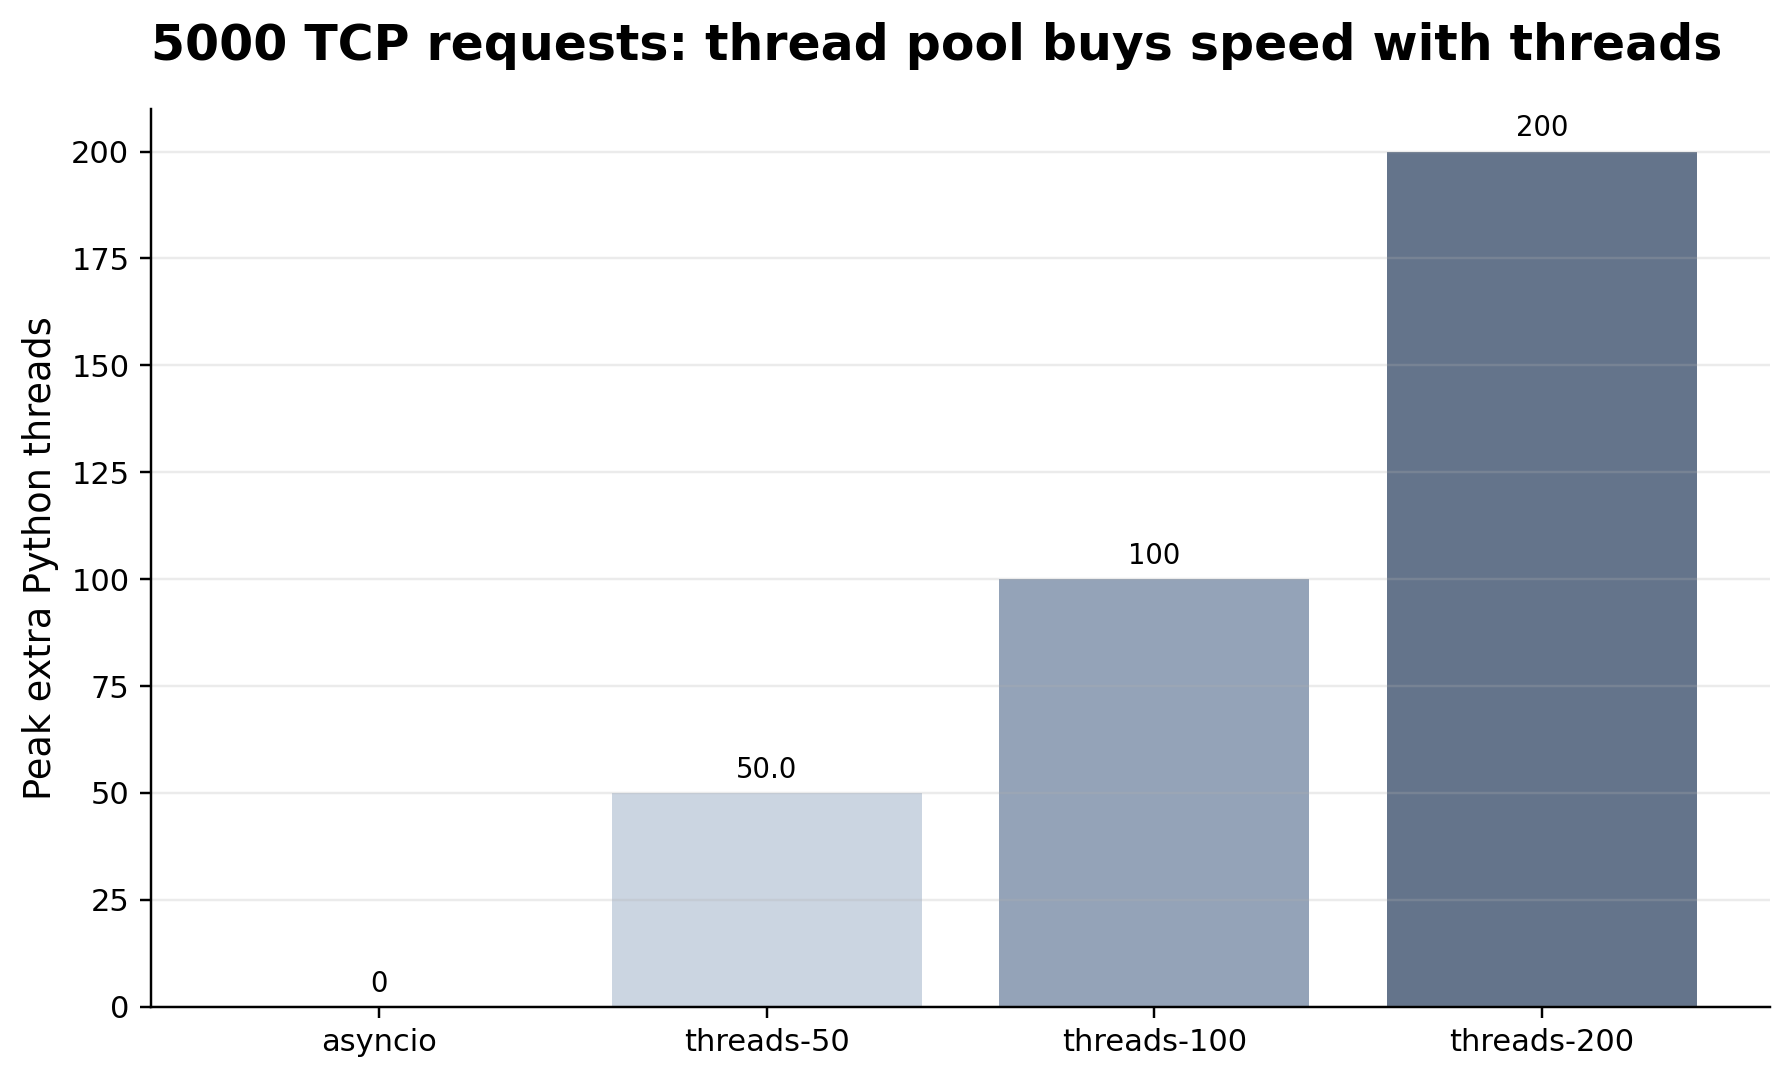
\includegraphics[keepaspectratio,alt={I/O线程峰值}]{assets/exp_io_thread_bar.png}}
\caption{I/O线程峰值}
\end{figure}

\begin{figure}
\centering
\pandocbounded{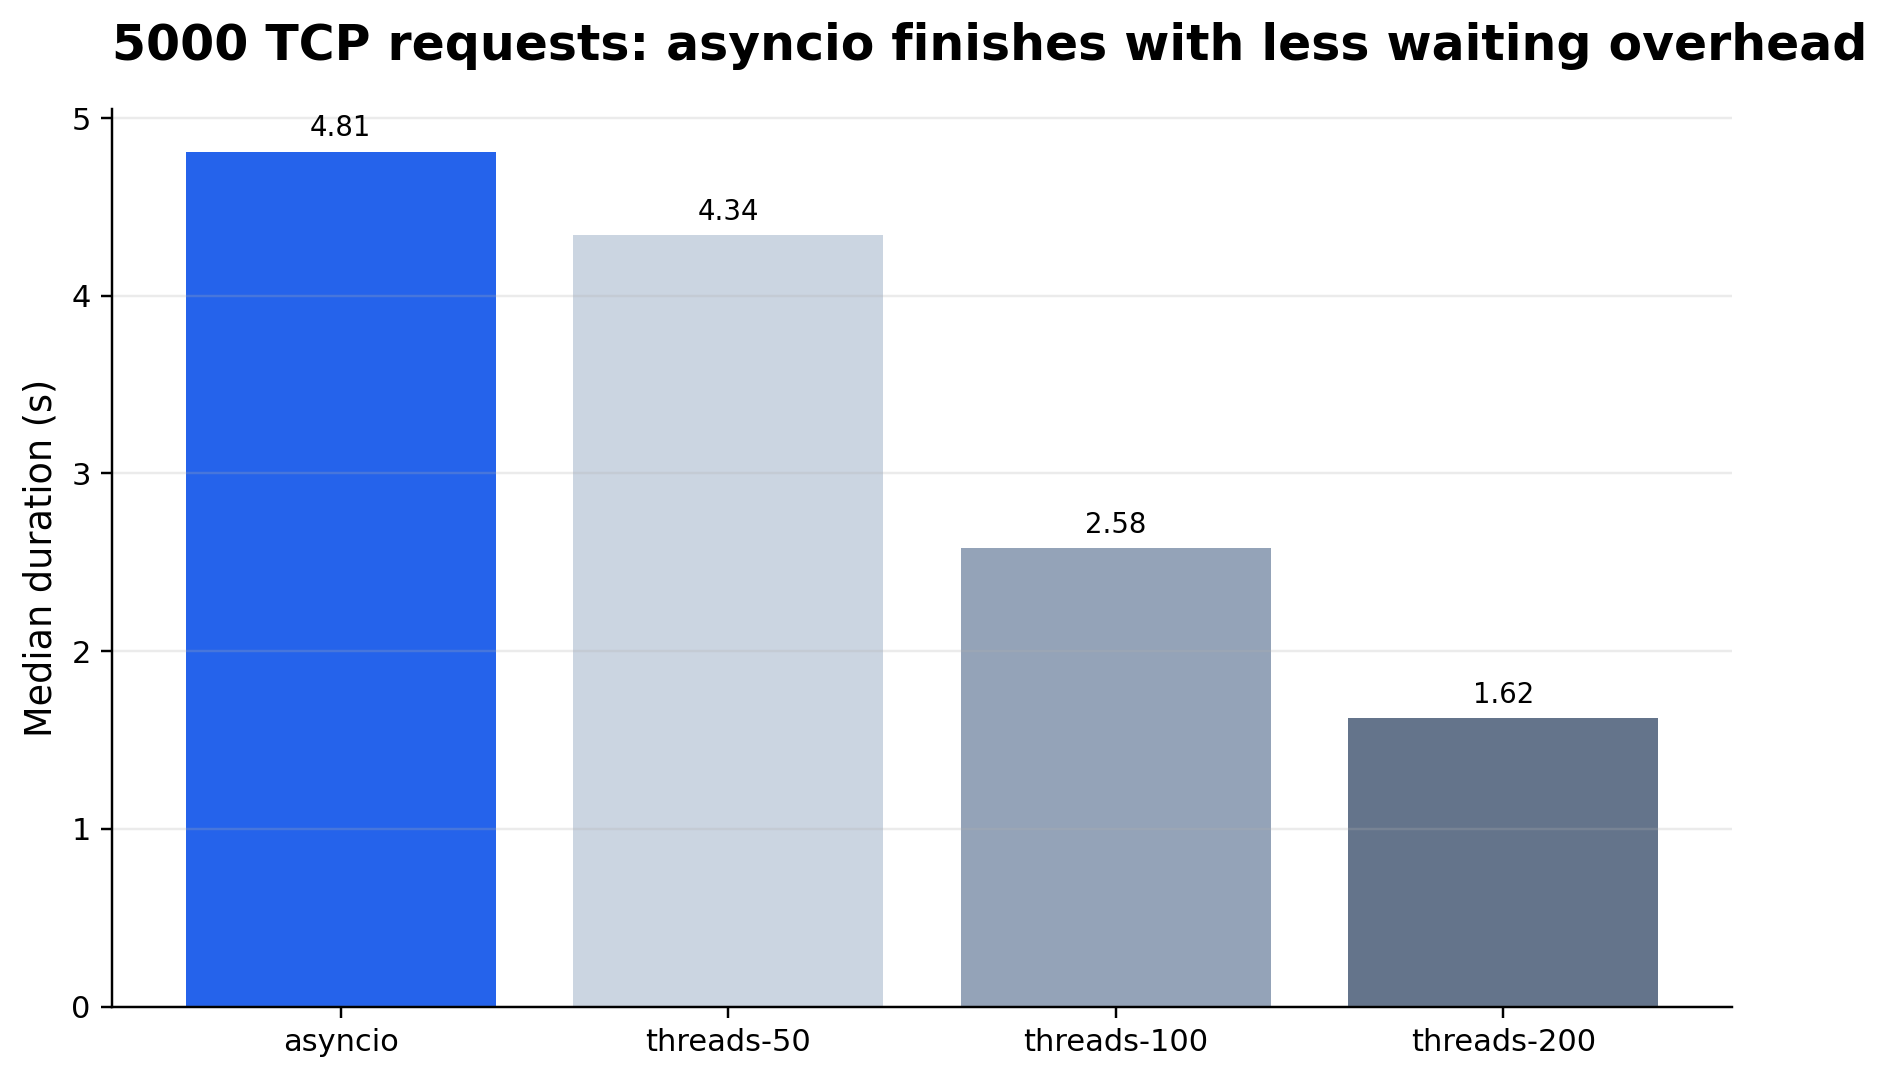
\includegraphics[keepaspectratio,alt={I/O耗时}]{assets/exp_io_duration_bar.png}}
\caption{I/O耗时}
\end{figure}

\subsection{5.2 I/O
扩展性与倍率}\label{io-ux6269ux5c55ux6027ux4e0eux500dux7387}

只比较 asyncio 与 threads-200，可以看到 threads-200
在延迟上更低，但这是用大量线程换来的结果。

\begin{figure}
\centering
\pandocbounded{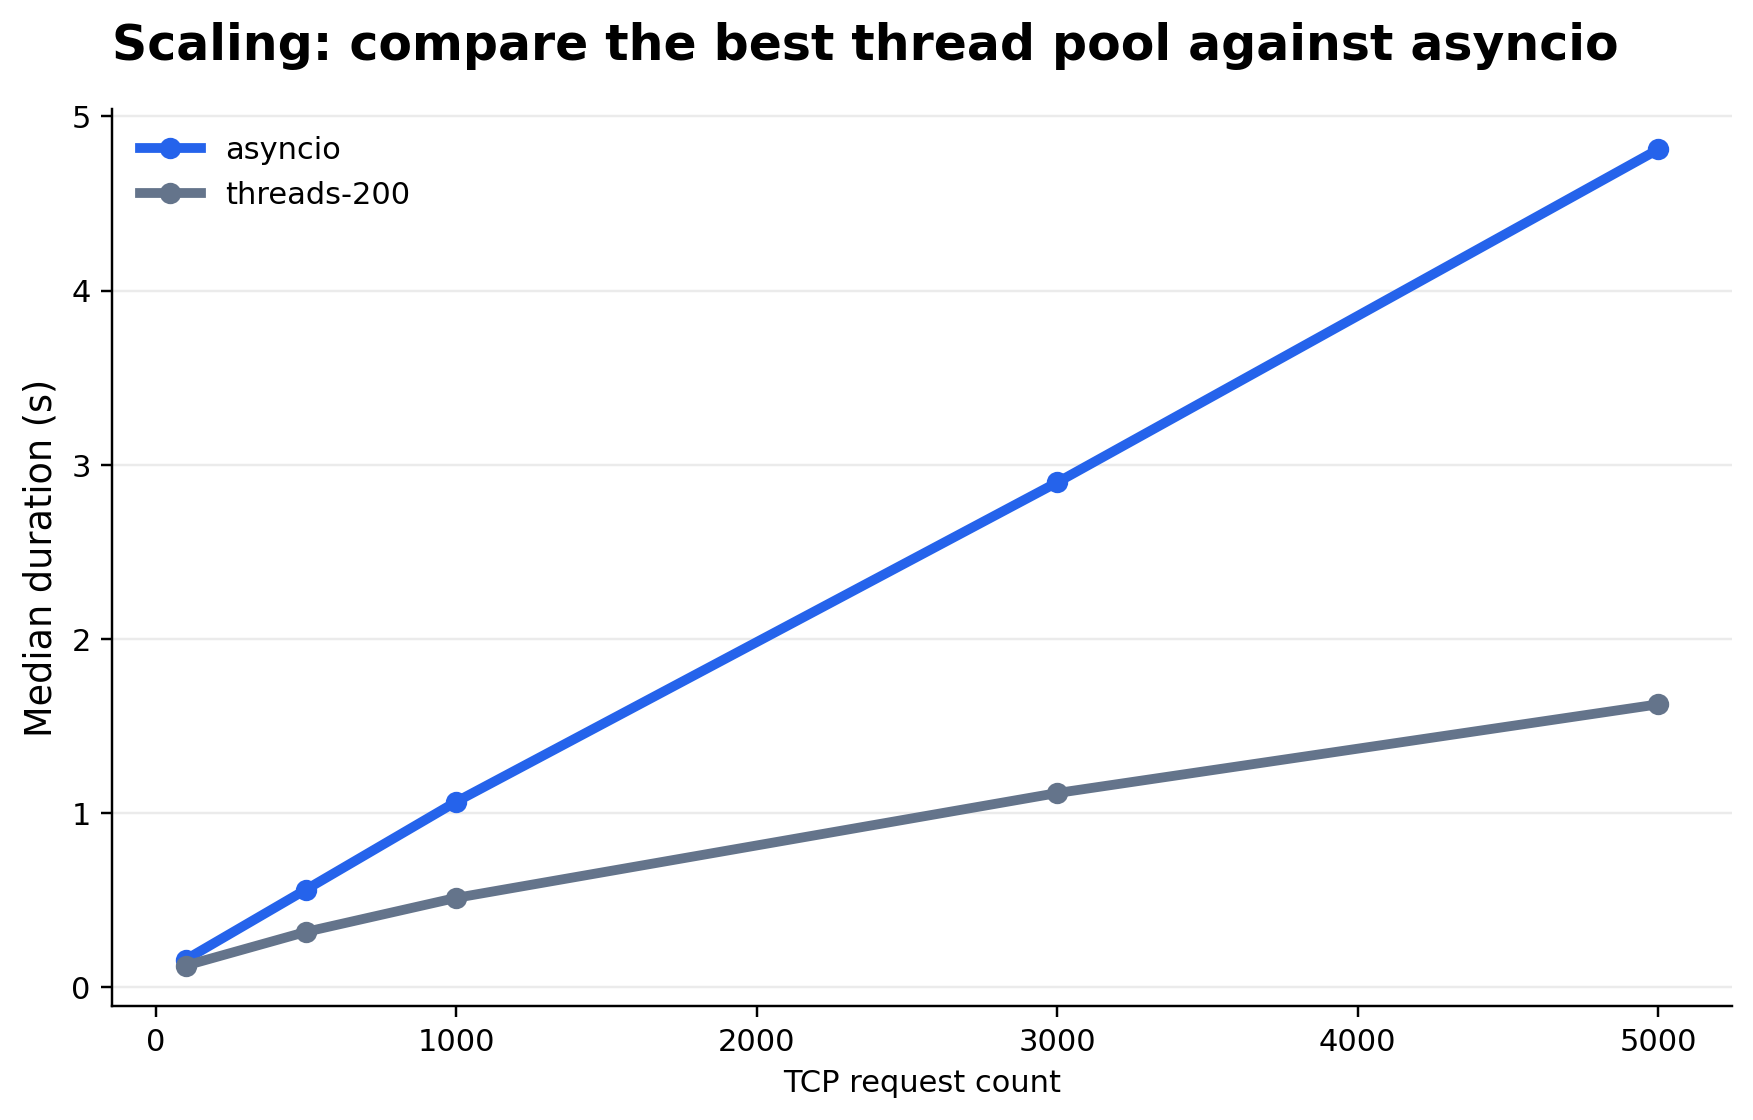
\includegraphics[keepaspectratio,alt={I/O扩展性}]{assets/exp_io_scaling_async_vs_thread200.png}}
\caption{I/O扩展性}
\end{figure}

\begin{figure}
\centering
\pandocbounded{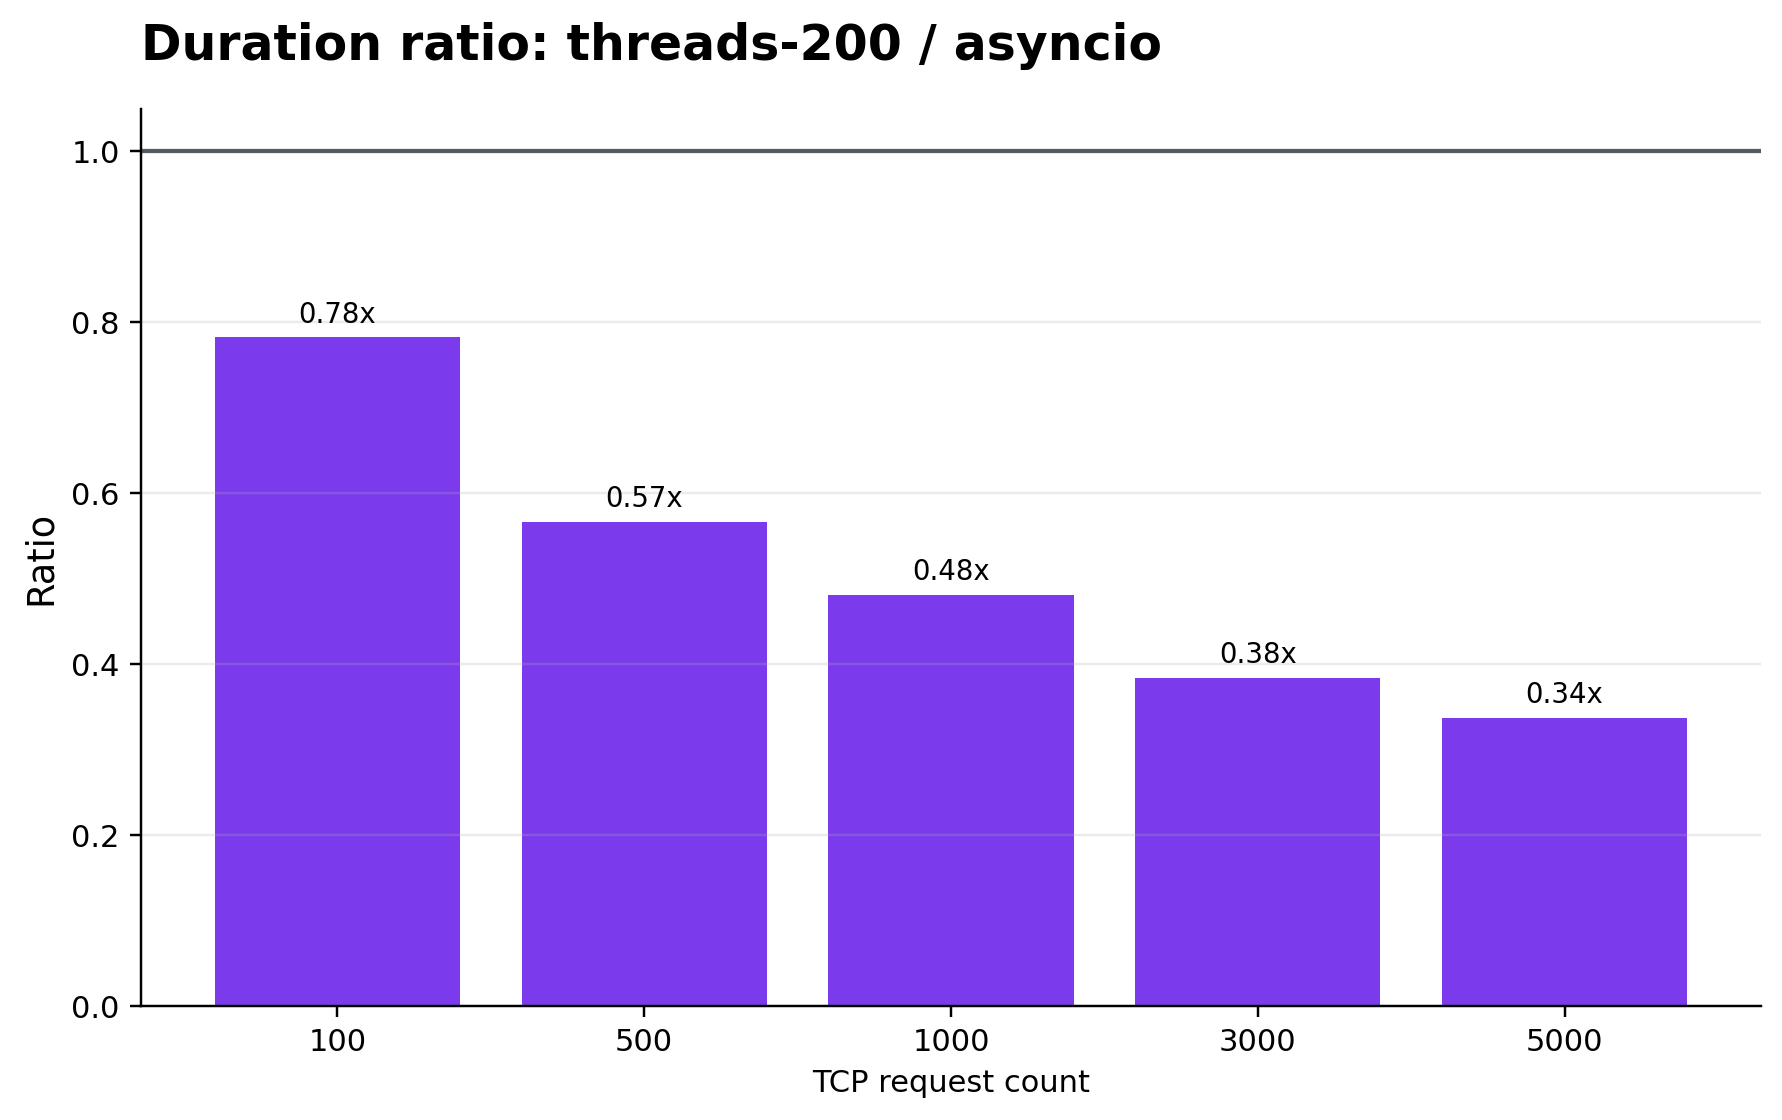
\includegraphics[keepaspectratio,alt={I/O耗时倍率}]{assets/exp_io_ratio.png}}
\caption{I/O耗时倍率}
\end{figure}

因此，正确的实验结论应该是：

\begin{itemize}
\tightlist
\item
  协程与线程池的耗时关系取决于并发规模、worker 数量、I/O
  特征和运行时实现；
\item
  协程的核心价值是用更少业务线程组织大量等待任务；
\item
  线程池可以通过增加 worker
  获得低延迟，但线程数、调度成本、内存和下游资源压力会同步上升；
\item
  工程选型应同时比较耗时、线程数、内存和下游容量。
\end{itemize}

\subsection{5.3 CPU-bound
场景：协程优势消失}\label{cpu-bound-ux573aux666fux534fux7a0bux4f18ux52bfux6d88ux5931}

在 200 个 CPU 计算任务中，各模型归一化耗时接近。

\begin{figure}
\centering
\pandocbounded{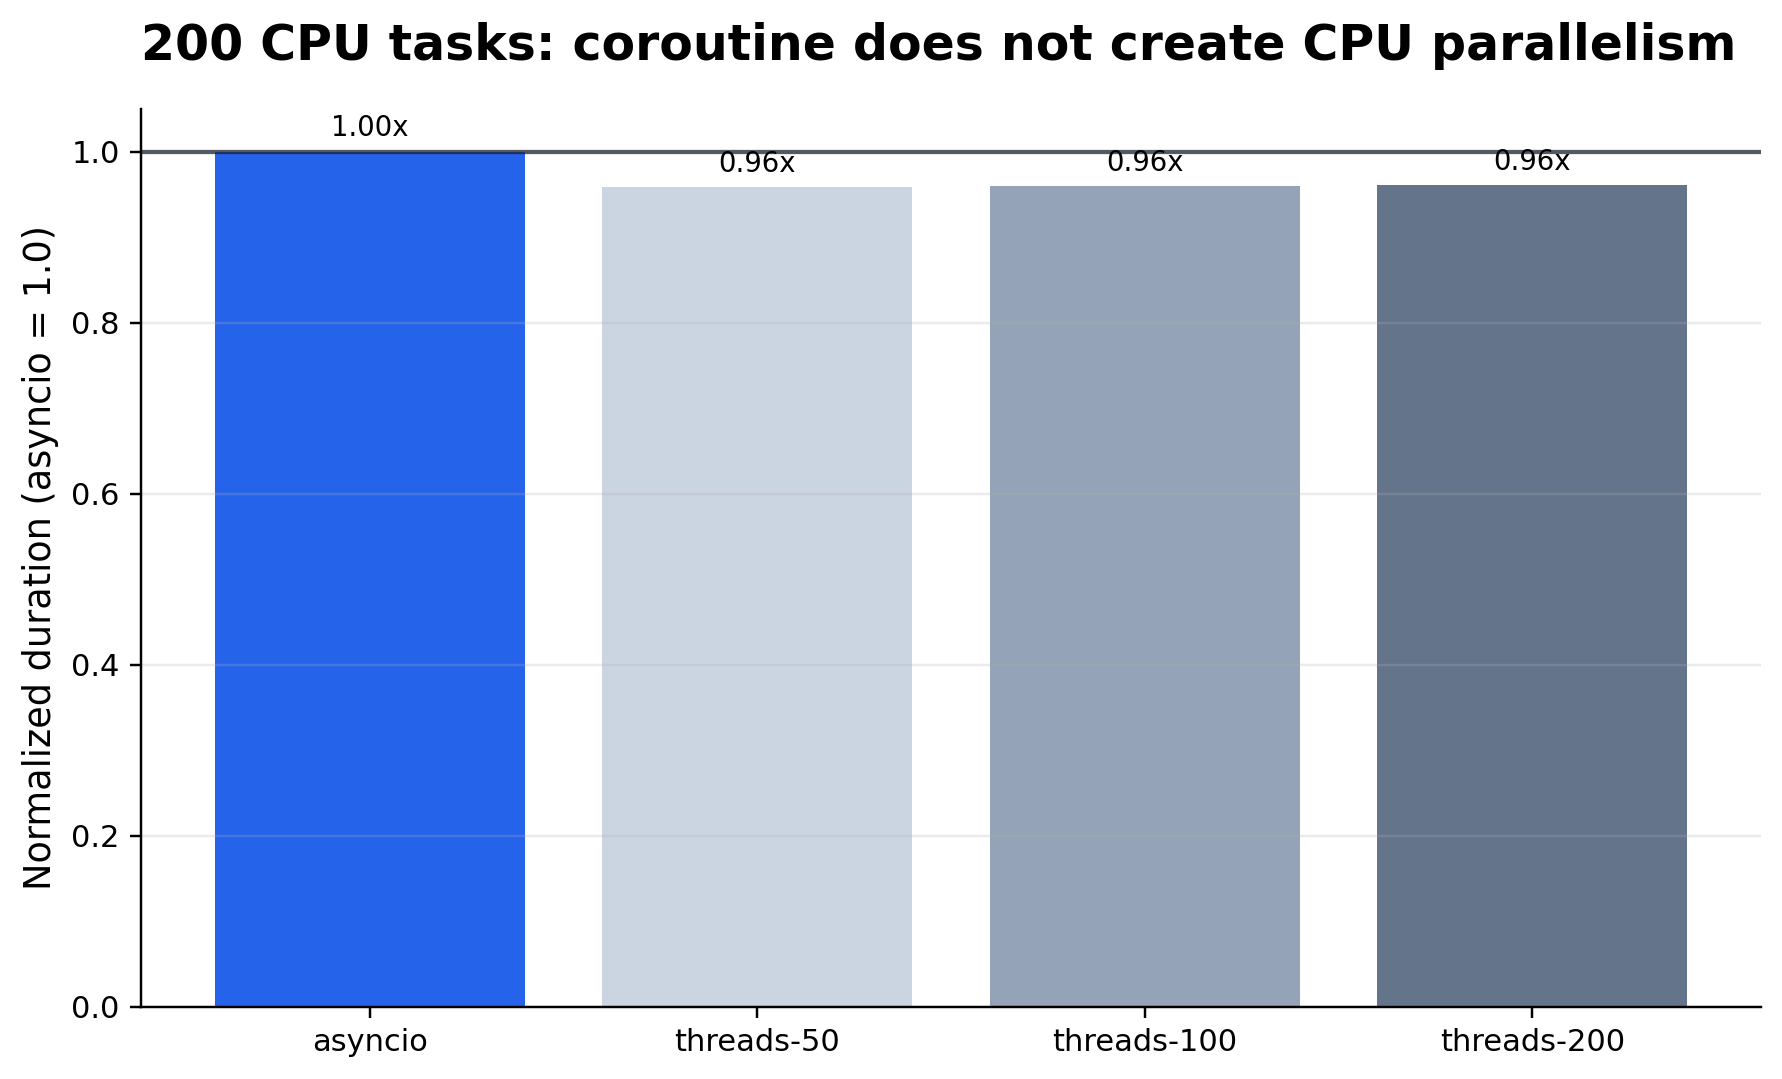
\includegraphics[keepaspectratio,alt={CPU归一化耗时}]{assets/exp_cpu_normalized_duration.png}}
\caption{CPU归一化耗时}
\end{figure}

这说明：

\begin{itemize}
\tightlist
\item
  CPU-bound 任务放入协程后仍受 CPU 核心数和计算实现限制；
\item
  Python 多线程受 GIL 和调度开销影响，对纯 Python CPU
  循环的加速能力有限；
\item
  CPU 密集任务应考虑进程池、C/C++/Rust 扩展、NumPy 向量化、SIMD、GPU
  或其他并行计算系统。
\end{itemize}

\section{6.
工程实践与常见问题}\label{ux5de5ux7a0bux5b9eux8df5ux4e0eux5e38ux89c1ux95eeux9898}

\subsection{6.1
适合使用协程的场景}\label{ux9002ux5408ux4f7fux7528ux534fux7a0bux7684ux573aux666f}

\begin{itemize}
\tightlist
\item
  高并发 Web 服务；
\item
  RPC、API 网关、下游聚合；
\item
  爬虫和批量 HTTP 请求；
\item
  数据库、缓存、消息队列访问；
\item
  WebSocket、IM、推送等长连接服务；
\item
  大量定时器和超时控制。
\end{itemize}

\subsection{6.2
协程收益有限的场景}\label{ux534fux7a0bux6536ux76caux6709ux9650ux7684ux573aux666f}

\begin{itemize}
\tightlist
\item
  纯 CPU 计算；
\item
  依赖大量阻塞式第三方库且无法替换；
\item
  强实时调度任务；
\item
  需要进程级隔离或崩溃隔离的任务；
\item
  无界创建任务且没有限流、背压和取消机制的系统。
\end{itemize}

\subsection{6.3
工程实践清单}\label{ux5de5ux7a0bux5b9eux8df5ux6e05ux5355}

推荐做法：

\begin{itemize}
\tightlist
\item
  给外部调用设置超时；
\item
  使用结构化并发管理任务生命周期；
\item
  对并发数设置上限，例如 semaphore、连接池、令牌桶；
\item
  明确取消传播和资源清理；
\item
  CPU 密集逻辑移出事件循环；
\item
  建立监控：任务数、队列长度、事件循环延迟、超时率、取消率、下游错误率。
\end{itemize}

\Needspace{8\baselineskip}

避免：

\begin{itemize}
\tightlist
\item
  无限创建 coroutine、Task 或 goroutine；
\item
  在事件循环中直接调用阻塞函数；
\item
  忽略取消后的资源清理；
\item
  只测平均耗时，不看尾延迟和资源成本；
\item
  误把协程当成``比线程更快的计算单元''。
\end{itemize}

\section{7. 局限性}\label{ux5c40ux9650ux6027}

本报告实验有以下局限：

\begin{itemize}
\tightlist
\item
  本地 loopback TCP 实验与公网生产环境存在网络路径、延迟和系统负载差异；
\item
  Windows 本地大量短连接会受到临时端口与 TIME\_WAIT
  限制，因此实验使用持久连接复用请求；
\item
  Python asyncio 和 Python 线程实验结论聚焦模型边界，不用于预测
  Go、Java、C++ 的具体性能；
\item
  RSS 采样会受到 Python 解释器、内存分配器和系统后台活动影响；
\item
  CPU-bound 实验受 Python GIL 影响，主要用于说明``协程不创造 CPU
  算力''，不用于评价其他语言的多线程 CPU 性能。
\end{itemize}

这些局限明确了结论的适用范围：协程适合降低 I/O 等待任务的线程占用，CPU
密集任务需要并行计算方案。

\section{8. AI 使用说明}\label{ai-ux4f7fux7528ux8bf4ux660e}

本项目中 AI 用于：

\begin{itemize}
\tightlist
\item
  根据课程要求梳理 PPT 结构；
\item
  搜集和归纳官方文档、PEP、JEP、语言文档和工程资料；
\item
  审阅实验设计是否能支撑结论；
\item
  改进实验脚本、生成图表和总结实验边界；
\item
  生成 SVG/PPTX/PDF 初稿。
\end{itemize}

\section{9. 参考资料}\label{ux53c2ux8003ux8d44ux6599}

\begingroup
\footnotesize

\begin{itemize}
\tightlist
\item
  \href{https://openjdk.org/jeps/444}{OpenJDK JEP 444: Virtual Threads}
\item
  \href{https://docs.python.org/3/library/asyncio-task.html}{Python
  asyncio Coroutines and Tasks}
\item
  \href{https://peps.python.org/pep-0492/}{PEP 492: Coroutines with
  async and await syntax}
\item
  \href{https://peps.python.org/pep-3156/}{PEP 3156: Asynchronous IO
  Support Rebooted}
\item
  \href{https://go.dev/doc/effective_go\#goroutines}{Go Effective Go:
  Goroutines}
\item
  \href{https://go.dev/ref/spec\#Go_statements}{Go language
  specification: Go statements}
\item
  \href{https://go.dev/src/runtime/HACKING.md}{Go runtime HACKING.md}
\item
  \href{https://learn.microsoft.com/en-us/dotnet/csharp/asynchronous-programming/}{Microsoft
  Learn: Asynchronous programming with async and await}
\item
  \href{https://learn.microsoft.com/en-us/dotnet/csharp/asynchronous-programming/async-scenarios}{Microsoft
  Learn: Async scenarios}
\item
  \href{https://en.cppreference.com/w/cpp/language/coroutines}{C++
  reference: Coroutines}
\item
  \href{https://eel.is/c++draft/dcl.fct.def.coroutine}{C++ draft
  coroutine section}
\item
  \href{https://llvm.org/docs/Coroutines.html}{LLVM Coroutines}
\item
  \href{https://man7.org/linux/man-pages/man7/epoll.7.html}{Linux epoll
  man page}
\item
  \href{https://learn.microsoft.com/en-us/windows/win32/fileio/i-o-completion-ports}{Microsoft
  I/O Completion Ports}
\item
  \href{https://docs.libuv.org/en/v1.x/design.html}{libuv Design
  overview}
\item
  \href{https://www.kegel.com/c10k.html}{The C10K problem}
\item
  \href{https://www.nginx.com/blog/inside-nginx-how-we-designed-for-performance-scale/}{NGINX
  performance and scale architecture}
\end{itemize}

\endgroup

\end{document}
